\subsection{Scenario and model} \label{sec:lv_scenario}
The scenario for the Local View model is represented in Figure \ref{fig:lv_scenario}. 

\begin{figure}[h!]
	\centering
	\subfloat[Local View model scenario (example)]{
		\includegraphics[width=0.4\textwidth]{images/model/LV_scenario}
		\label{fig:lv_scenario}
	}
	\subfloat[Real and binary sensing models]{
		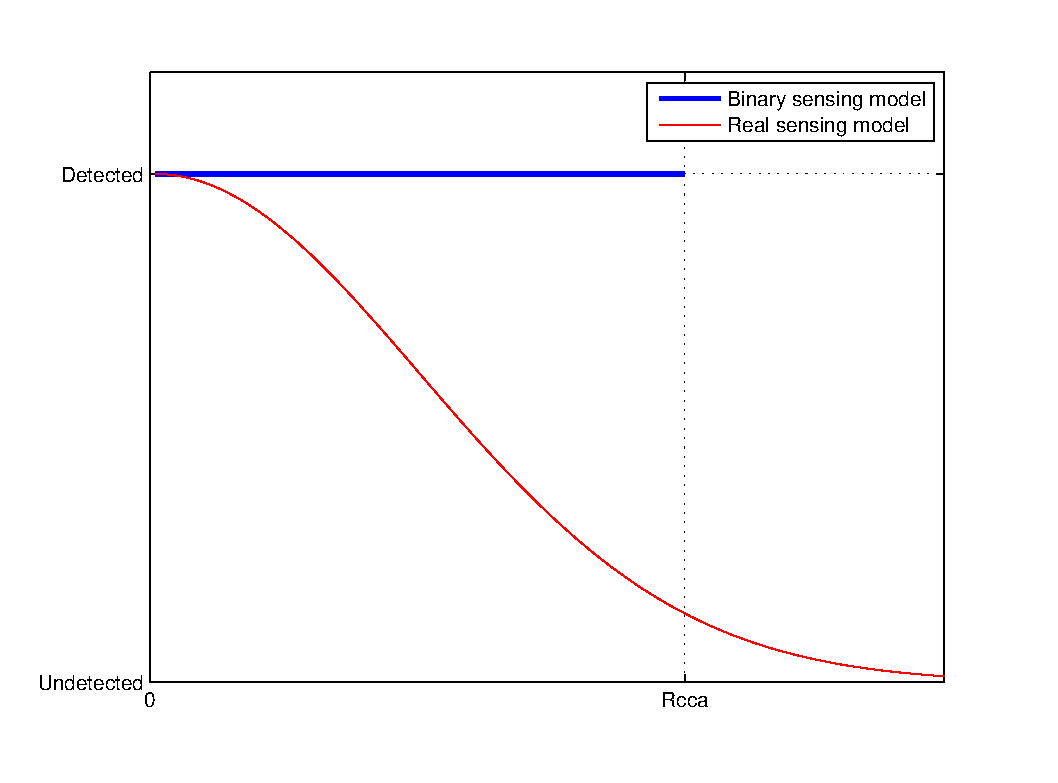
\includegraphics[width=0.5\textwidth]{images/model/binary}
		\label{fig:lv_sensing_binary}
	}
	\caption{Local View model scenario and sensing model}
	\label{fig:lv_scenario_and_sensing}
\end{figure}

We define a binary sensing model in which the activity of all the \acs{WLAN} users within the sensor's sensing range will be detected while the ones outside this sensing area will not be observed (Figure \ref{fig:lv_sensing_binary}). However, the real sensing model will decrease its sensing capability gradually. The sensing area of the sensor is denoted as Clear Channel Assessment (\acs{CCA}) zone.

Because of this limited sensing range, each sensor distributed in the scenario will observe a different portion of the spectrum activity generated by the nodes within its sensing range and therefore, estimate its own parameters from the observed activity. This issue requires an extension of the two-state semi-Markovian model presented in Figure \ref{fig:semi-markov} in order to represent the unseen activity of the nodes outside the sensing range. The parameters estimated in each one of the sensor can differ depending on the traffic scheme generated by the sensed nodes.

The new semi-Markovian model is composed by three states: idle, active observed and active unseen, represented in Figure \ref{fig:semi-markov_local}. 

\begin{figure}[h]
	\centering
	\includegraphics[scale=0.5]{images/model/semi-markov_lv}
	\caption{Semi-markovian model \cite{marcello}}
	\label{fig:semi-markov_local}
\end{figure}

It is necessary to define a new parameter that reflects the portion or percentage of traffic seen and unseen. The parameter $P_{cca}$ determines the probability of detected \acs{WLAN} activity. Consequently, $1-P_{cca}$ represents the portion of unseen activity.

The active distribution for this new three-state semi-Markovian model is represented by the same active distribution used in the Global View model: uniform distribution. The estimation of the parameters for the active distribution $\alpha_{ON}$ and $\beta_{ON}$ are estimated by the shortest and largest measured active periods respectively, as it was done in the Global View model. On the other hand, the Global View idle distribution cannot be used in this Local View since the sensor skips a portion of the active periods in the network \cite{marcello}. For this, the estimation of the parameters cannot be done in the same way as before as it is presented in \cite{marcello}. The local idle distribution is a combination of the global idle distribution, the active distribution and the observable load $P_{cca}$ and cannot be expressed in a closed form, which do not allow to apply the \acs{MLE} estimation process presented in \cite{marcello-thesis}.

Three different approaches have been presented in \cite{marcello} and \cite{marcello-thesis} to estimate the idle distribution parameters for the Local View model: compound \acs{MLE}/\acs{ME}, Laplace Estimation and Neural Networks. We will focus on the Laplace estimation, which is revised in the following section.